% Generated by paper/tools/update_experiment_results.py from results/exp.md.
\section{Additional Experimental Results}

\label{app:experimental_results}

\subsection{Coverage and Comparison Scope}

\label{app:result_coverage}

All primary conditions target the same 354 conversations and 1,404 rubric items. A small number of judgments remained unavailable because of API failures and are not re-run. Marginal results use available judgments, whereas paired and factorial analyses use the corresponding comparison-specific common sets, so their denominators can differ from one another and from the marginal tables. Marginal tables report point estimates, and conversation-level bootstrap intervals accompany the headline contrasts (Appendix~\ref{app:bootstrap_ci}).

The evaluation uses AudioMC's fixed-context, binary-rubric protocol, but our rubric success pools criteria within each language. AudioMC's average rubric score first averages within each conversation; these aggregations differ when conversations have unequal numbers of criteria. Survival conditions on reference-passing paired rubric items. Transcription gains and recovery use comparison-specific common conversation sets. Recovery is the fraction of reference-success/audio-failure conversations that an intervention makes successful; it does not count new failures introduced elsewhere and should be read alongside net paired gain.

Historical assistant responses remain fixed text in every procedure: models generate only the designated response, rather than an online rollout of their own conversation histories.

Additional transcript-source diagnostics and implementation exceptions are described in Appendix~\ref{app:transcript_sources}.

Avg. is the ten-language macro mean (English human recordings plus nine non-English languages); the paired-comparison gains of Appendix~\ref{app:transcript_sources} lack an English export and their Avg. is the nine non-English languages, as noted in their captions. Std. is the population standard deviation and Range is the maximum minus minimum, both in percentage points. These dispersion measures use the reported language scores, rounded to one decimal place, and do not measure sampling uncertainty. A dash denotes unavailable results rather than zero.

% Generated by paper/tools/update_experiment_results.py from results/exp.md.
\begin{table}[p]
\centering
\caption{Direct-audio results in all ten languages. Each cell reports \textbf{rubric / instance} success (\%). EN uses human speech; other languages use synthesized speech. Bold denotes the best displayed value separately for each metric, language, and capability. Overall aggregates all items, not the four capability percentages. Some runs have incomplete scoring; see Appendix~\ref{app:result_coverage}.}
\label{tab:audio_complete}
\begingroup
\fontsize{8.2}{9.8}\selectfont
\setlength{\tabcolsep}{1pt}
\renewcommand{\arraystretch}{1.06}
\begin{tabular*}{\linewidth}{@{}l@{\hspace{3pt}\extracolsep{\fill}}*{10}{r}@{}}
\toprule
\multicolumn{11}{@{}l}{\textbf{(a) Inference Memory (IM)}} \\
\textbf{Model} & \textbf{EN} & \textbf{ZH} & \textbf{JA} & \textbf{ES} & \textbf{FR} & \textbf{RU} & \textbf{DE} & \textbf{IT} & \textbf{TH} & \textbf{VI} \\
\midrule
Qwen3.8 Omni & 72.5/58.5 & \textbf{74.5}/\textbf{61.0} & \textbf{75.2}/\textbf{61.0} & \textbf{79.1}/\textbf{67.1} & \textbf{73.9}/\textbf{61.0} & \textbf{73.9}/\textbf{61.0} & \textbf{73.2}/\textbf{62.2} & \textbf{73.2}/\textbf{61.0} & \textbf{69.3}/\textbf{53.7} & \textbf{66.0}/\textbf{51.2} \\
Gemini 3.1 Pro & \textbf{75.2}/\textbf{59.8} & 60.8/43.9 & 66.0/48.8 & 64.7/51.2 & 68.0/50.0 & 69.3/52.4 & 64.7/48.8 & 66.0/51.2 & 68.0/\textbf{53.7} & 60.1/43.9 \\
Gemini 3.8 Flash & 72.5/\textbf{59.8} & 64.1/47.6 & 64.1/47.6 & 62.7/43.9 & 63.4/46.3 & 68.6/56.1 & 66.0/50.0 & 64.7/51.2 & 65.4/46.3 & 57.5/39.0 \\
Doubao Seed Lite & 65.4/47.6 & 64.7/48.8 & 58.2/43.9 & 60.1/42.7 & 60.8/42.7 & 70.6/52.4 & 70.6/50.0 & 62.7/46.3 & 52.3/37.8 & 58.2/40.2 \\
Qwen3.5 Omni & 55.6/34.1 & 47.1/32.9 & 60.1/42.7 & 56.2/41.5 & 51.6/34.1 & 58.2/40.2 & 56.2/34.1 & 58.8/42.7 & 55.6/31.7 & 47.7/28.0 \\
Muse-Spark 1.2 & 62.7/41.5 & 54.2/32.9 & 50.3/31.2 & 51.6/31.7 & 55.6/32.9 & 52.9/32.9 & 50.3/29.3 & 52.3/32.9 & 52.9/30.5 & 51.0/32.9 \\
\addlinespace[3pt]
\midrule
\multicolumn{11}{@{}l}{\textbf{(b) Instruction Retention (IR)}} \\
\textbf{Model} & \textbf{EN} & \textbf{ZH} & \textbf{JA} & \textbf{ES} & \textbf{FR} & \textbf{RU} & \textbf{DE} & \textbf{IT} & \textbf{TH} & \textbf{VI} \\
\midrule
Qwen3.8 Omni & \textbf{89.9}/\textbf{80.0} & \textbf{86.5}/\textbf{69.6} & \textbf{83.8}/\textbf{66.3} & \textbf{86.0}/\textbf{75.8} & \textbf{89.2}/\textbf{78.9} & \textbf{83.8}/\textbf{67.4} & \textbf{87.4}/\textbf{75.8} & \textbf{87.4}/\textbf{75.8} & \textbf{83.1}/\textbf{65.3} & \textbf{85.6}/\textbf{71.6} \\
Gemini 3.1 Pro & 81.3/71.6 & 72.3/57.9 & 65.1/54.7 & 78.8/67.4 & 74.8/66.3 & 80.6/61.1 & 72.7/63.2 & 82.4/66.3 & 65.8/53.7 & 76.6/64.2 \\
Gemini 3.8 Flash & 75.9/54.7 & 71.6/54.7 & 66.2/48.4 & 73.4/61.1 & 69.8/52.6 & 72.3/53.7 & 73.0/51.6 & 77.0/57.9 & 64.7/46.3 & 70.1/48.4 \\
Doubao Seed Lite & 75.2/53.7 & 73.0/51.6 & 65.5/45.3 & 71.2/49.5 & 68.3/47.4 & 67.6/48.4 & 70.5/45.3 & 69.8/54.7 & 63.3/44.2 & 67.6/43.2 \\
Qwen3.5 Omni & 66.2/50.5 & 62.9/45.3 & 60.1/42.1 & 67.3/45.3 & 62.9/45.3 & 66.9/45.3 & 64.4/44.2 & 66.2/43.2 & 58.6/42.1 & 64.0/42.1 \\
Muse-Spark 1.2 & 66.9/53.7 & 43.2/24.2 & 36.1/22.3 & 56.5/43.2 & 55.4/36.8 & 56.1/43.2 & 55.4/40.0 & 54.7/36.8 & 37.8/21.1 & 43.5/27.4 \\
\addlinespace[3pt]
\midrule
\multicolumn{11}{@{}l}{\textbf{(c) Self Coherence (SC)}} \\
\textbf{Model} & \textbf{EN} & \textbf{ZH} & \textbf{JA} & \textbf{ES} & \textbf{FR} & \textbf{RU} & \textbf{DE} & \textbf{IT} & \textbf{TH} & \textbf{VI} \\
\midrule
Qwen3.8 Omni & \textbf{82.3}/\textbf{41.6} & \textbf{81.4}/\textbf{49.4} & 77.9/\textbf{50.6} & \textbf{83.3}/\textbf{48.1} & \textbf{80.4}/\textbf{40.3} & 80.4/45.5 & \textbf{81.1}/\textbf{48.1} & \textbf{80.4}/\textbf{42.9} & \textbf{77.9}/36.4 & \textbf{83.0}/\textbf{48.1} \\
Gemini 3.1 Pro & 76.0/40.3 & 79.8/42.9 & \textbf{81.1}/48.1 & 77.6/44.2 & 74.8/\textbf{40.3} & \textbf{81.7}/46.8 & 77.0/37.7 & 77.9/40.3 & 70.7/32.5 & 76.0/36.4 \\
Gemini 3.8 Flash & 72.9/32.5 & 77.0/40.3 & 71.0/40.3 & 76.7/39.0 & 75.1/36.4 & 77.3/40.3 & 76.3/41.6 & 70.3/33.8 & 72.2/40.3 & 72.9/33.8 \\
Doubao Seed Lite & 72.2/29.9 & 73.5/37.7 & 71.6/36.4 & 64.0/26.0 & 67.2/26.0 & 69.4/31.2 & 66.2/27.3 & 67.8/24.7 & 64.0/28.6 & 66.6/26.0 \\
Qwen3.5 Omni & 77.0/37.7 & 78.2/40.3 & 71.0/35.1 & 72.6/31.2 & 73.5/35.1 & 73.5/28.6 & 74.8/37.7 & 69.7/29.9 & 70.3/32.5 & 69.7/32.5 \\
Muse-Spark 1.2 & 76.3/40.3 & 73.5/39.0 & 67.2/42.9 & 70.3/37.7 & 74.1/35.1 & \textbf{81.7}/\textbf{50.6} & 78.2/39.0 & 75.4/40.3 & 69.4/\textbf{41.6} & 69.1/37.7 \\
\addlinespace[3pt]
\midrule
\multicolumn{11}{@{}l}{\textbf{(d) Voice Editing (VE)}} \\
\textbf{Model} & \textbf{EN} & \textbf{ZH} & \textbf{JA} & \textbf{ES} & \textbf{FR} & \textbf{RU} & \textbf{DE} & \textbf{IT} & \textbf{TH} & \textbf{VI} \\
\midrule
Qwen3.8 Omni & 90.9/62.0 & \textbf{89.6}/\textbf{61.0} & \textbf{90.4}/\textbf{62.0} & \textbf{90.4}/63.0 & 88.4/55.0 & \textbf{92.1}/\textbf{67.0} & 89.5/58.0 & 88.0/\textbf{60.0} & \textbf{88.3}/57.0 & 87.2/\textbf{59.0} \\
Gemini 3.1 Pro & \textbf{91.3}/\textbf{65.0} & 87.0/56.0 & 90.2/59.0 & 89.9/\textbf{64.0} & \textbf{90.1}/\textbf{59.0} & 90.1/63.0 & \textbf{89.9}/\textbf{61.0} & \textbf{89.3}/\textbf{60.0} & 87.8/\textbf{58.0} & \textbf{88.9}/57.0 \\
Gemini 3.8 Flash & 87.7/58.0 & 89.2/\textbf{61.0} & 88.6/56.0 & 87.8/58.0 & 86.1/57.0 & 88.4/60.0 & 87.2/57.0 & 87.5/59.0 & 85.5/57.0 & 84.6/53.0 \\
Doubao Seed Lite & 87.7/56.0 & 83.5/46.0 & 82.0/42.0 & 83.2/41.0 & 84.1/46.0 & 81.4/47.0 & 82.5/42.0 & 84.6/49.0 & 81.4/42.0 & 81.9/33.0 \\
Qwen3.5 Omni & 84.1/47.0 & 82.5/40.0 & 79.6/35.0 & 80.8/35.0 & 81.2/34.0 & 81.1/38.0 & 79.6/34.0 & 82.6/37.0 & 80.5/37.0 & 79.6/31.0 \\
Muse-Spark 1.2 & 67.1/25.0 & 56.2/21.4 & 61.7/24.2 & 69.8/25.0 & 67.4/26.0 & 67.2/27.0 & 65.0/27.3 & 71.8/22.2 & 60.2/19.0 & 60.1/18.2 \\
\addlinespace[3pt]
\midrule
\multicolumn{11}{@{}l}{\textbf{(e) Overall}} \\
\textbf{Model} & \textbf{EN} & \textbf{ZH} & \textbf{JA} & \textbf{ES} & \textbf{FR} & \textbf{RU} & \textbf{DE} & \textbf{IT} & \textbf{TH} & \textbf{VI} \\
\midrule
Qwen3.8 Omni & \textbf{86.8}/\textbf{61.6} & \textbf{85.5}/\textbf{60.7} & \textbf{84.6}/\textbf{60.5} & \textbf{86.7}/\textbf{64.1} & \textbf{85.2}/\textbf{59.6} & \textbf{85.8}/\textbf{61.0} & \textbf{85.4}/\textbf{61.6} & \textbf{84.5}/\textbf{60.7} & \textbf{82.8}/\textbf{54.0} & \textbf{83.6}/\textbf{58.2} \\
Gemini 3.1 Pro & 84.1/60.2 & 79.6/50.8 & 80.6/53.1 & 82.2/57.6 & 81.2/54.8 & 84.0/56.5 & 80.8/53.7 & 82.8/55.4 & 77.4/50.3 & 80.4/51.4 \\
Gemini 3.8 Flash & 80.3/52.0 & 80.2/51.7 & 77.5/48.6 & 79.7/51.4 & 77.9/48.9 & 80.6/53.1 & 79.6/50.6 & 79.1/51.4 & 76.2/48.0 & 76.1/44.4 \\
Doubao Seed Lite & 79.3/47.7 & 77.1/46.3 & 73.8/42.1 & 74.0/40.4 & 74.6/41.2 & 74.8/45.2 & 75.1/41.5 & 75.5/44.6 & 70.7/38.7 & 73.0/35.9 \\
Qwen3.5 Omni & 75.9/42.9 & 73.8/39.8 & 71.7/38.7 & 73.6/38.4 & 72.6/37.3 & 74.1/38.4 & 72.9/37.6 & 73.9/38.4 & 71.2/36.2 & 70.8/33.6 \\
Muse-Spark 1.2 & 68.7/39.8 & 57.3/28.7 & 56.6/29.4 & 65.3/34.2 & 65.2/32.5 & 66.7/37.9 & 64.5/33.7 & 67.0/32.6 & 57.1/27.1 & 57.9/28.3 \\
\bottomrule
\end{tabular*}
\endgroup
\end{table}


\subsection{Full Factorial Results}

\label{app:full_factorial_results}

The full instance-level and rubric-level factorial results behind the marginal contrasts of Table~\ref{tab:input_conditions} appear in Tables~\ref{tab:instance_conditions} and~\ref{tab:rubric_conditions}; Appendix~\ref{app:factorial_details} details the four-condition comparison scope, and Figure~\ref{fig:transcription_gains} visualizes the language-level contrasts.

% Generated by paper/tools/update_experiment_results.py from results/exp.md.
\begin{table}[htbp]
\centering
\caption{Overall instance success (\%) by language and input condition. Avg. is the ten-language macro mean (English human recordings included). Entries use available judgments. Condition definitions and scoring exceptions appear in Appendix~\ref{app:result_coverage}.}
\label{tab:instance_conditions}
\begingroup
\fontsize{8.2}{9.1}\selectfont
\setlength{\tabcolsep}{1pt}
\renewcommand{\arraystretch}{1.06}
\begin{tabular*}{\linewidth}{@{}ll@{\extracolsep{\fill}}*{11}{r}@{}}
\toprule
\textbf{Model} & \textbf{Input} & \textbf{Avg.} & \textbf{EN} & \textbf{ZH} & \textbf{JA} & \textbf{ES} & \textbf{FR} & \textbf{RU} & \textbf{DE} & \textbf{IT} & \textbf{TH} & \textbf{VI} \\
\midrule
Qwen3.8 Omni & Reference Transcript & 60.9 & 61.6 & 62.4 & 58.9 & 66.7 & 59.6 & 63.0 & 64.4 & 60.7 & 50.8 & 61.3 \\
 & Direct Audio & 60.2 & 61.6 & 60.7 & 60.5 & 64.1 & 59.6 & 61.0 & 61.6 & 60.7 & 54.0 & 58.2 \\
 & History Transcript & 60.1 & 60.2 & 61.8 & 62.0 & 60.5 & 59.6 & 63.3 & 61.9 & 61.6 & 54.0 & 55.6 \\
 & Current Transcript & 60.1 & 62.7 & 59.0 & 61.0 & 63.0 & 62.1 & 62.1 & 63.0 & 62.4 & 51.1 & 54.8 \\
 & Full Transcript & 58.8 & 62.4 & 60.7 & 59.4 & 61.9 & 62.4 & 61.9 & 59.6 & 57.6 & 48.6 & 53.4 \\
\addlinespace[1pt]
\midrule
Gemini 3.1 Pro & Reference Transcript & 63.0 & 63.0 & 65.5 & 65.0 & 64.1 & 63.3 & 60.5 & 63.3 & 63.3 & 61.9 & 59.6 \\
 & Direct Audio & 54.4 & 60.2 & 50.8 & 53.1 & 57.6 & 54.8 & 56.5 & 53.7 & 55.4 & 50.3 & 51.4 \\
 & History Transcript & 60.1 & 64.1 & 58.5 & 61.9 & 61.9 & 59.0 & 62.1 & 60.2 & 58.8 & 57.3 & 57.3 \\
 & Current Transcript & 57.1 & 60.8 & 57.5 & 55.8 & 58.2 & 58.2 & 58.2 & 57.9 & 57.1 & 52.3 & 55.4 \\
 & Full Transcript & 60.8 & 66.9 & 61.3 & 62.7 & 61.6 & 59.6 & 60.7 & 59.0 & 61.3 & 56.8 & 58.2 \\
\addlinespace[1pt]
\midrule
Gemini 3.8 Flash & Reference Transcript & 57.0 & 59.3 & 58.8 & 57.9 & 54.5 & 54.5 & 56.5 & 58.8 & 56.8 & 55.9 & 56.5 \\
 & Direct Audio & 50.0 & 52.0 & 51.7 & 48.6 & 51.4 & 48.9 & 53.1 & 50.6 & 51.4 & 48.0 & 44.4 \\
 & History Transcript & 53.2 & 58.8 & 55.1 & 48.3 & 54.8 & 50.6 & 56.8 & 54.0 & 52.3 & 49.4 & 52.0 \\
 & Current Transcript & 50.8 & 55.1 & 54.0 & 49.6 & 49.6 & 51.1 & 52.5 & 50.6 & 52.1 & 46.2 & 46.7 \\
 & Full Transcript & 54.4 & 57.8 & 56.2 & 52.8 & 55.4 & 54.5 & 57.9 & 54.5 & 54.8 & 49.4 & 50.6 \\
\addlinespace[1pt]
\midrule
Doubao Seed Lite & Reference Transcript & 48.4 & 46.9 & 50.6 & 50.6 & 49.2 & 46.9 & 48.9 & 47.2 & 48.3 & 45.2 & 50.3 \\
 & Direct Audio & 42.4 & 47.7 & 46.3 & 42.1 & 40.4 & 41.2 & 45.2 & 41.5 & 44.6 & 38.7 & 35.9 \\
 & History Transcript & 45.1 & 51.1 & 50.0 & 47.7 & 44.1 & 43.5 & 46.3 & 43.5 & 44.6 & 40.7 & 39.5 \\
 & Current Transcript & 43.4 & 48.0 & 45.2 & 43.8 & 42.4 & 44.9 & 44.1 & 44.4 & 44.4 & 38.7 & 38.4 \\
 & Full Transcript & 46.3 & 50.3 & 46.3 & 49.7 & 42.9 & 45.5 & 46.0 & 43.8 & 48.3 & 42.7 & 47.2 \\
\addlinespace[1pt]
\midrule
Qwen3.5 Omni & Reference Transcript & 40.1 & 42.4 & 41.0 & 41.0 & 41.5 & 40.4 & 40.4 & 39.3 & 39.3 & 35.3 & 40.4 \\
 & Direct Audio & 38.1 & 42.9 & 39.8 & 38.7 & 38.4 & 37.3 & 38.4 & 37.6 & 38.4 & 36.2 & 33.6 \\
 & History Transcript & 39.8 & 42.7 & 41.9 & 37.9 & 40.4 & 39.5 & 42.1 & 39.8 & 42.2 & 37.6 & 33.6 \\
 & Current Transcript & 38.4 & 42.7 & 41.8 & 37.3 & 39.3 & 39.0 & 39.5 & 36.4 & 35.7 & 35.3 & 36.7 \\
 & Full Transcript & 38.1 & 39.5 & 38.1 & 38.4 & 37.9 & 40.4 & 40.7 & 36.7 & 40.1 & 33.6 & 35.9 \\
\addlinespace[1pt]
\midrule
Muse-Spark 1.2 & Reference Transcript & 64.0 & 64.7 & 62.4 & 64.0 & 63.8 & 66.7 & 67.5 & 65.0 & 63.6 & 61.3 & 60.9 \\
 & Direct Audio & 32.4 & 39.8 & 28.7 & 29.4 & 34.2 & 32.5 & 37.9 & 33.7 & 32.6 & 27.1 & 28.3 \\
 & History Transcript & 52.5 & 55.9 & 46.6 & 50.4 & 55.5 & 54.2 & 55.6 & 55.6 & 54.1 & 48.3 & 49.2 \\
 & Current Transcript & 38.6 & 45.2 & 32.8 & 38.1 & 42.1 & 40.4 & 39.8 & 42.1 & 42.2 & 31.2 & 32.5 \\
 & Full Transcript & 58.6 & 58.5 & 58.6 & 55.6 & 60.2 & 60.5 & 64.7 & 61.9 & 60.2 & 55.4 & 50.3 \\
\bottomrule
\end{tabular*}
\endgroup
\end{table}


% Generated by paper/tools/update_experiment_results.py from results/exp.md.
\begin{table}[htbp]
\centering
\caption{Overall rubric success (\%) by language and input condition. Avg. is the ten-language macro mean (English human recordings included). Entries use available judgments. Condition definitions and scoring exceptions appear in Appendix~\ref{app:result_coverage}.}
\label{tab:rubric_conditions}
\begingroup
\fontsize{8.2}{9.1}\selectfont
\setlength{\tabcolsep}{1pt}
\renewcommand{\arraystretch}{1.06}
\begin{tabular*}{\linewidth}{@{}ll@{\extracolsep{\fill}}*{11}{r}@{}}
\toprule
\textbf{Model} & \textbf{Input} & \textbf{Avg.} & \textbf{EN} & \textbf{ZH} & \textbf{JA} & \textbf{ES} & \textbf{FR} & \textbf{RU} & \textbf{DE} & \textbf{IT} & \textbf{TH} & \textbf{VI} \\
\midrule
Qwen3.8 Omni & Reference Transcript & 85.7 & 85.6 & 86.2 & 84.6 & 88.0 & 85.4 & 86.5 & 87.3 & 84.6 & 82.1 & 86.8 \\
 & Direct Audio & 85.1 & 86.8 & 85.5 & 84.6 & 86.7 & 85.2 & 85.8 & 85.4 & 84.5 & 82.8 & 83.6 \\
 & History Transcript & 84.7 & 85.2 & 85.8 & 84.2 & 85.8 & 84.3 & 85.6 & 85.2 & 85.1 & 82.1 & 83.3 \\
 & Current Transcript & 84.9 & 86.9 & 84.3 & 84.5 & 86.4 & 86.0 & 85.8 & 86.1 & 85.4 & 80.5 & 83.2 \\
 & Full Transcript & 84.5 & 85.9 & 85.2 & 85.1 & 86.4 & 86.5 & 85.6 & 85.2 & 83.0 & 78.6 & 83.6 \\
\addlinespace[1pt]
\midrule
Gemini 3.1 Pro & Reference Transcript & 86.1 & 87.1 & 87.1 & 87.0 & 87.1 & 86.1 & 85.1 & 86.7 & 86.2 & 83.6 & 85.0 \\
 & Direct Audio & 81.3 & 84.1 & 79.6 & 80.6 & 82.2 & 81.2 & 84.0 & 80.8 & 82.8 & 77.4 & 80.4 \\
 & History Transcript & 84.6 & 87.1 & 84.9 & 84.8 & 85.8 & 84.4 & 85.2 & 84.7 & 84.0 & 81.6 & 83.9 \\
 & Current Transcript & 83.3 & 85.2 & 82.6 & 83.1 & 83.8 & 83.9 & 84.1 & 83.9 & 82.8 & 79.8 & 83.3 \\
 & Full Transcript & 84.6 & 88.2 & 84.5 & 85.3 & 85.4 & 84.3 & 85.0 & 85.0 & 83.6 & 81.3 & 83.8 \\
\addlinespace[1pt]
\midrule
Gemini 3.8 Flash & Reference Transcript & 82.5 & 84.3 & 82.8 & 82.6 & 82.5 & 80.8 & 82.7 & 82.5 & 82.4 & 81.7 & 82.9 \\
 & Direct Audio & 78.7 & 80.3 & 80.2 & 77.5 & 79.7 & 77.9 & 80.6 & 79.6 & 79.1 & 76.2 & 76.1 \\
 & History Transcript & 80.5 & 83.0 & 80.4 & 78.1 & 81.5 & 79.0 & 81.8 & 81.1 & 80.8 & 78.1 & 81.2 \\
 & Current Transcript & 79.6 & 82.2 & 81.7 & 78.8 & 79.7 & 79.8 & 80.8 & 79.2 & 79.5 & 76.6 & 77.6 \\
 & Full Transcript & 81.4 & 83.3 & 82.4 & 80.8 & 83.0 & 81.4 & 83.4 & 81.6 & 80.1 & 77.6 & 79.9 \\
\addlinespace[1pt]
\midrule
Doubao Seed Lite & Reference Transcript & 78.5 & 78.7 & 79.0 & 78.6 & 80.3 & 77.6 & 78.4 & 77.4 & 78.1 & 76.7 & 80.1 \\
 & Direct Audio & 74.8 & 79.3 & 77.1 & 73.8 & 74.0 & 74.6 & 74.8 & 75.1 & 75.5 & 70.7 & 73.0 \\
 & History Transcript & 76.8 & 80.9 & 78.4 & 77.1 & 77.0 & 75.9 & 76.2 & 76.6 & 75.6 & 74.1 & 75.7 \\
 & Current Transcript & 75.6 & 79.2 & 76.6 & 75.0 & 76.1 & 75.9 & 75.3 & 76.7 & 76.7 & 72.4 & 72.1 \\
 & Full Transcript & 77.4 & 79.9 & 78.6 & 77.1 & 75.6 & 77.4 & 76.8 & 76.7 & 78.3 & 75.8 & 77.3 \\
\addlinespace[1pt]
\midrule
Qwen3.5 Omni & Reference Transcript & 73.7 & 76.0 & 75.2 & 71.2 & 74.8 & 73.7 & 73.7 & 73.5 & 73.4 & 70.2 & 75.3 \\
 & Direct Audio & 73.1 & 75.9 & 73.8 & 71.7 & 73.6 & 72.6 & 74.1 & 72.9 & 73.9 & 71.2 & 70.8 \\
 & History Transcript & 73.5 & 75.4 & 73.0 & 70.2 & 74.3 & 72.9 & 75.3 & 74.6 & 75.2 & 71.5 & 72.6 \\
 & Current Transcript & 73.1 & 75.1 & 74.0 & 72.2 & 72.6 & 74.1 & 74.7 & 73.1 & 71.6 & 69.3 & 74.6 \\
 & Full Transcript & 72.9 & 75.5 & 73.2 & 71.1 & 72.5 & 73.2 & 74.6 & 73.8 & 73.3 & 69.5 & 72.6 \\
\addlinespace[1pt]
\midrule
Muse-Spark 1.2 & Reference Transcript & 86.0 & 86.9 & 85.1 & 85.9 & 86.3 & 86.9 & 87.3 & 86.9 & 86.2 & 83.9 & 85.0 \\
 & Direct Audio & 62.6 & 68.7 & 57.3 & 56.6 & 65.3 & 65.2 & 66.7 & 64.5 & 67.0 & 57.1 & 57.9 \\
 & History Transcript & 79.9 & 82.2 & 77.5 & 77.7 & 82.5 & 78.9 & 81.6 & 81.6 & 81.6 & 77.3 & 78.4 \\
 & Current Transcript & 70.6 & 74.9 & 67.1 & 69.1 & 72.8 & 70.8 & 72.2 & 73.0 & 72.8 & 65.8 & 67.4 \\
 & Full Transcript & 83.2 & 83.0 & 83.5 & 82.2 & 84.6 & 82.5 & 85.4 & 85.0 & 84.5 & 79.8 & 81.2 \\
\bottomrule
\end{tabular*}
\endgroup
\end{table}


\subsubsection{History--Current Contrasts and Scoring Scope}

\label{app:factorial_details}

The two input factors are preceding user history and the current user turn. With A denoting audio and T the frozen model-generated transcript, (A,A) is Direct Audio, (T,A) is History Transcript, (A,T) is Current Transcript, and (T,T) is Full Transcript. Historical assistant responses remain fixed text. The text substitutions reuse the same frozen transcripts. Reference Transcript and reference-history inputs are separate controls, not cells of this factorial design.

All contrasts in Table~\ref{tab:factorial_effects} are computed from the marginal instance scores in Tables~\ref{tab:input_conditions} and~\ref{tab:instance_conditions}. History and Current are the two single-substitution contrasts relative to Direct Audio; Full substitutes both. The arithmetic interaction TT$-$TA$-$AT$+$AA equals Full$-$History$-$Current. Positive values indicate a larger full-substitution contrast than the sum of the two single substitutions; negative values indicate a smaller one. Neither sign establishes an internal processing mechanism.

Marginal condition scores and contrasts in Tables~\ref{tab:input_conditions} and~\ref{tab:instance_conditions} use available judgments. To separate scoring coverage from intervention effects, Appendix~\ref{app:bootstrap_ci} re-estimates each headline contrast on its corresponding complete common set; the factorial interaction is computed on the intersection complete across Direct Audio, History Transcript, Current Transcript, and Full Transcript. Its interval spans zero for five of the six models and lies below zero for Gemini 3.1 Pro ($-2.1$ points, 95\% CI $[-4.1, -0.03]$, whose upper endpoint rounds to zero at the table's integer precision), so interaction size and stability remain unestablished and additivity is a point-estimate observation. Current Transcript is reported at the Overall level in the marginal tables; the recovery-overlap analysis of Appendix~\ref{app:recovery_overlap} compares its conversation-level rescues with History Transcript on the four-arm common set.

% Generated by paper/tools/update_experiment_results.py from results/exp.md.
\begin{table}[htbp]
\centering
\caption{Transcript substitutions in the $2\times2$ design: ten-language macro-mean instance-score contrasts (pp). History, Current and Full subtract Direct Audio from History Transcript, Current Transcript and Full Transcript, respectively. Interaction is Full$-$History$-$Current. These are \textbf{marginal contrasts}, not common-set paired effects.}
\label{tab:factorial_effects}
\begingroup
\fontsize{8.5}{10.5}\selectfont
\setlength{\tabcolsep}{1pt}
\renewcommand{\arraystretch}{1.06}
\begin{tabular*}{0.76\linewidth}{@{}l@{\extracolsep{\fill}}rrrr@{}}
\toprule
\textbf{Model} & \textbf{History} & \textbf{Current} & \textbf{Full} & \textbf{Interaction} \\
\midrule
Qwen3.8 Omni & -0.2 & -0.1 & -1.4 & -1.2 \\
Gemini 3.1 Pro & +5.7 & +2.8 & +6.4 & -2.1 \\
Gemini 3.8 Flash & +3.2 & +0.7 & +4.4 & +0.4 \\
Doubao Seed Lite & +2.7 & +1.1 & +3.9 & +0.1 \\
Qwen3.5 Omni & +1.6 & +0.2 & 0.0 & -1.9 \\
Muse-Spark 1.2 & +20.1 & +6.2 & +26.2 & -0.2 \\
\bottomrule
\end{tabular*}
\endgroup
\end{table}


The main-text Table~\ref{tab:input_conditions} summarizes the average marginal contrasts; the tables below retain the per-language history/current contrasts and interaction details.

% Generated by paper/tools/update_experiment_results.py from results/exp.md.
\begin{table}[htbp]
\centering
\caption{Language-level history / current substitution contrasts in instance success (pp), each relative to marginal Direct Audio. Avg. is the ten-language macro mean (English human recordings included); individual language values use the reported rounded scores. These are descriptive contrasts on available judgments.}
\label{tab:factorial_languages}
\begingroup
\fontsize{6.6}{8.2}\selectfont
\setlength{\tabcolsep}{1pt}
\renewcommand{\arraystretch}{1.06}
\begin{tabular*}{\linewidth}{@{}l@{\extracolsep{\fill}}*{11}{r}@{}}
\toprule
\textbf{Model} & \textbf{Avg.} & \textbf{EN} & \textbf{ZH} & \textbf{JA} & \textbf{ES} & \textbf{FR} & \textbf{RU} & \textbf{DE} & \textbf{IT} & \textbf{TH} & \textbf{VI} \\
\midrule
Qwen3.8 Omni & -0.2/-0.1 & -1.4/+1.1 & +1.1/-1.7 & +1.5/+0.5 & -3.6/-1.1 & 0.0/+2.5 & +2.3/+1.1 & +0.3/+1.4 & +0.9/+1.7 & 0.0/-2.9 & -2.6/-3.4 \\
Gemini 3.1 Pro & +5.7/+2.8 & +3.9/+0.6 & +7.7/+6.7 & +8.8/+2.7 & +4.3/+0.6 & +4.2/+3.4 & +5.6/+1.7 & +6.5/+4.2 & +3.4/+1.7 & +7.0/+2.0 & +5.9/+4.0 \\
Gemini 3.8 Flash & +3.2/+0.7 & +6.8/+3.1 & +3.4/+2.3 & -0.3/+1.0 & +3.4/-1.8 & +1.7/+2.2 & +3.7/-0.6 & +3.4/0.0 & +0.9/+0.7 & +1.4/-1.8 & +7.6/+2.3 \\
Doubao Seed Lite & +2.7/+1.1 & +3.4/+0.3 & +3.7/-1.1 & +5.6/+1.7 & +3.7/+2.0 & +2.3/+3.7 & +1.1/-1.1 & +2.0/+2.9 & 0.0/-0.2 & +2.0/0.0 & +3.6/+2.5 \\
Qwen3.5 Omni & +1.6/+0.2 & -0.2/-0.2 & +2.1/+2.0 & -0.8/-1.4 & +2.0/+0.9 & +2.2/+1.7 & +3.7/+1.1 & +2.2/-1.2 & +3.8/-2.7 & +1.4/-0.9 & 0.0/+3.1 \\
Muse-Spark 1.2 & +20.1/+6.2 & +16.1/+5.4 & +17.9/+4.1 & +21.0/+8.7 & +21.3/+7.9 & +21.7/+7.9 & +17.7/+1.9 & +21.9/+8.4 & +21.5/+9.6 & +21.2/+4.1 & +20.9/+4.2 \\
\bottomrule
\end{tabular*}
\endgroup
\end{table}



\begin{figure}[htbp]

\centering

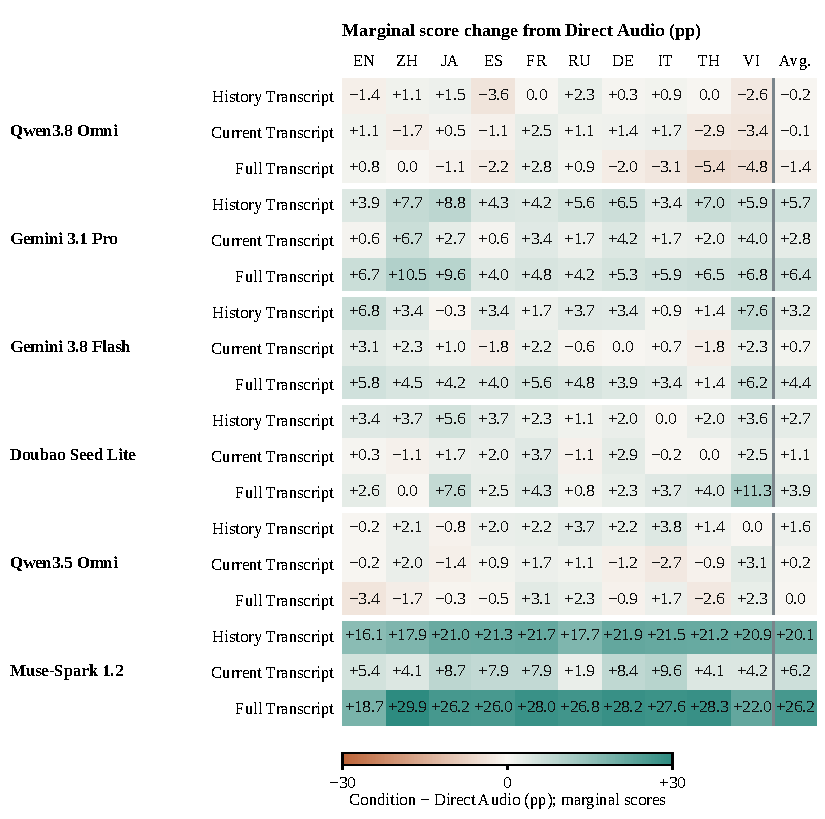
\includegraphics[width=\linewidth]{figures/factorial_gains.pdf}

\caption{Language-level marginal instance-success contrasts with Direct Audio (pp). All six models appear in the Table~\ref{tab:input_conditions} order, with three rows each: History Transcript, Current Transcript, and Full Transcript. EN is first; Avg. is the ten-language macro mean (English human recordings included). Contrasts use available judgments rather than a common four-condition set. The same contrasts appear numerically in Table~\ref{tab:factorial_languages}.}

\label{fig:transcription_gains}

\end{figure}

\subsection{Conversation-Level Bootstrap Intervals}

\label{app:bootstrap_ci}

The headline contrasts are re-estimated by resampling source conversations rather than rubric items. A conversation counts as successful only when every rubric judged for it succeeds, matching the instance scores used elsewhere. Each model block draws one bag-of-source-conversations resample and applies the same sampled conversation identifiers to all ten language versions and all conditions, so the intervals exploit the parallel multilingual structure instead of treating the ten language versions of one source conversation as independent samples. Each contrast is computed on its own comparison-specific common set per language: the conditions involved in that contrast are jointly complete, and Reference Transcript therefore never restricts the factorial contrasts. The reported point estimates are these common-set estimates; the marginal estimates in Tables~\ref{tab:modality_summary} and~\ref{tab:input_conditions} use available judgments and can differ slightly.

The resulting intervals appear in Table~\ref{tab:bootstrap_ci}. Intervals use 10{,}000 replicates and report the 2.5th--97.5th percentiles; the 10-lang. column averages the per-language replicate contrasts with English human recordings included. These intervals measure benchmark-sample uncertainty over the observed conversations. They do not cover generation stochasticity; judge-family robustness is assessed in Appendix~\ref{app:judge_robustness}.

% Generated by paper/tools/update_experiment_results.py from results/exp.md.
\begin{table}[t]
\centering
\caption{Ninety-five percent conversation-level bootstrap intervals (pp) for six contrasts: Ref.$-$Direct, History, Current, and Full each subtract Direct Audio; H$-$C is History minus Current; Interaction is Full$-$History$-$Current$+$Direct. Each contrast uses its own comparison-specific common set per language (322 to 354 conversations per language); source conversations are resampled jointly across the ten language versions, so the macro column reflects source-level uncertainty. The macro cell gives the common-set point estimate with 2.5--97.5 percentiles of 10{,}000 replicates; intervals cover benchmark-sample uncertainty only.}
\label{tab:bootstrap_ci}
\fontsize{7.0}{8.6}\selectfont
\setlength{\tabcolsep}{1.2pt}
\begin{tabular*}{\linewidth}{@{}l@{\hspace{5pt}}l@{\hspace{3pt}\extracolsep{\fill}}*{10}{r}@{\hspace{8pt}}r@{}}
\toprule
 & & \multicolumn{10}{c}{Per language (95\% CI)} & Macro \\
\cmidrule(lr){3-12}\cmidrule(lr){13-13}
\textbf{Model} & \textbf{Contrast} & \textbf{EN} & \textbf{ZH} & \textbf{JA} & \textbf{ES} & \textbf{FR} & \textbf{RU} & \textbf{DE} & \textbf{IT} & \textbf{TH} & \textbf{VI} & \textbf{10-lang.} \\
\midrule
Qwen3.8 Omni & Ref.$-$Direct & $-5$--$5$ & $-3$--$6$ & $-6$--$3$ & $-2$--$7$ & $-5$--$5$ & $-3$--$7$ & $-2$--$8$ & $-5$--$5$ & $-8$--$2$ & $-2$--$8$ & $+0.8$ [$-1$, $2$] \\
 & History & $-6$--$3$ & $-3$--$5$ & $-3$--$6$ & $-8$--$0$ & $-5$--$5$ & $-3$--$7$ & $-5$--$5$ & $-3$--$5$ & $-5$--$5$ & $-7$--$2$ & $0$ [$-2$, $1$] \\
 & Current & $-3$--$5$ & $-7$--$3$ & $-4$--$5$ & $-5$--$3$ & $-2$--$7$ & $-4$--$6$ & $-3$--$6$ & $-3$--$6$ & $-8$--$2$ & $-8$--$1$ & $0$ [$-1$, $1$] \\
 & Full & $-4$--$5$ & $-5$--$5$ & $-5$--$3$ & $-7$--$3$ & $-2$--$7$ & $-4$--$6$ & $-7$--$3$ & $-8$--$1$ & $-10$--$-1$ & $-10$--$0$ & $-1.4$ [$-3$, $0$] \\
 & H$-$C & $-7$--$2$ & $-2$--$8$ & $-4$--$5$ & $-6$--$1$ & $-7$--$2$ & $-3$--$6$ & $-6$--$3$ & $-5$--$3$ & $-2$--$8$ & $-4$--$5$ & $0$ [$-2$, $1$] \\
 & Interaction & $-5$--$7$ & $-6$--$7$ & $-10$--$3$ & $-3$--$8$ & $-6$--$6$ & $-9$--$4$ & $-10$--$3$ & $-12$--$0$ & $-9$--$4$ & $-5$--$7$ & $-1.2$ [$-3$, $1$] \\
\midrule
Gemini 3.1 Pro & Ref.$-$Direct & $-2$--$7$ & $10$--$20$ & $7$--$17$ & $2$--$11$ & $4$--$13$ & $-1$--$9$ & $5$--$14$ & $3$--$12$ & $7$--$16$ & $3$--$13$ & $+8.6$ [$6$, $11$] \\
 & History & $0$--$8$ & $3$--$12$ & $4$--$14$ & $0$--$9$ & $-1$--$9$ & $1$--$10$ & $2$--$11$ & $-1$--$8$ & $3$--$12$ & $1$--$11$ & $+5.7$ [$4$, $8$] \\
 & Current & $-4$--$5$ & $3$--$11$ & $-2$--$7$ & $-3$--$5$ & $-1$--$8$ & $-3$--$6$ & $0$--$8$ & $-3$--$6$ & $-3$--$6$ & $-1$--$8$ & $+2.8$ [$1$, $4$] \\
 & Full & $3$--$11$ & $6$--$15$ & $5$--$15$ & $-1$--$8$ & $0$--$10$ & $0$--$8$ & $1$--$10$ & $1$--$11$ & $1$--$12$ & $1$--$12$ & $+6.4$ [$4$, $9$] \\
 & H$-$C & $-1$--$8$ & $-4$--$6$ & $1$--$11$ & $-1$--$8$ & $-3$--$5$ & $-1$--$9$ & $-2$--$7$ & $-3$--$6$ & $0$--$10$ & $-2$--$6$ & $+3.0$ [$1$, $5$] \\
 & Interaction & $-3$--$8$ & $-10$--$1$ & $-8$--$4$ & $-6$--$5$ & $-9$--$3$ & $-9$--$3$ & $-11$--$0$ & $-4$--$6$ & $-8$--$3$ & $-9$--$3$ & $-2.1$ [$-4$, $0$] \\
\midrule
Gemini 3.8 Flash & Ref.$-$Direct & $2$--$12$ & $3$--$12$ & $5$--$14$ & $-2$--$8$ & $1$--$10$ & $-1$--$8$ & $3$--$13$ & $1$--$10$ & $4$--$12$ & $7$--$17$ & $+6.9$ [$5$, $9$] \\
 & History & $3$--$11$ & $-1$--$8$ & $-5$--$5$ & $-1$--$8$ & $-3$--$6$ & $-1$--$8$ & $-2$--$8$ & $-4$--$5$ & $-3$--$6$ & $3$--$13$ & $+3.2$ [$1$, $5$] \\
 & Current & $-2$--$8$ & $-3$--$7$ & $-3$--$5$ & $-7$--$3$ & $-2$--$7$ & $-5$--$4$ & $-5$--$5$ & $-3$--$5$ & $-6$--$3$ & $-2$--$7$ & $+0.8$ [$-1$, $2$] \\
 & Full & $1$--$10$ & $0$--$9$ & $-1$--$9$ & $-1$--$9$ & $1$--$10$ & $0$--$10$ & $-1$--$9$ & $-1$--$8$ & $-3$--$6$ & $1$--$11$ & $+4.4$ [$2$, $7$] \\
 & H$-$C & $-1$--$8$ & $-3$--$6$ & $-6$--$3$ & $0$--$10$ & $-5$--$4$ & $-1$--$9$ & $-2$--$8$ & $-5$--$5$ & $-1$--$8$ & $1$--$10$ & $+2.4$ [$1$, $4$] \\
 & Interaction & $-10$--$2$ & $-7$--$5$ & $-3$--$9$ & $-3$--$9$ & $-5$--$8$ & $-4$--$8$ & $-5$--$6$ & $-4$--$7$ & $-4$--$8$ & $-10$--$2$ & $0$ [$-2$, $2$] \\
\midrule
Doubao Seed Lite & Ref.$-$Direct & $-6$--$4$ & $-1$--$9$ & $4$--$13$ & $4$--$14$ & $1$--$10$ & $-1$--$9$ & $1$--$10$ & $-1$--$8$ & $2$--$11$ & $9$--$20$ & $+6.0$ [$4$, $8$] \\
 & History & $-2$--$8$ & $-1$--$8$ & $1$--$10$ & $0$--$8$ & $-2$--$6$ & $-4$--$6$ & $-3$--$7$ & $-5$--$5$ & $-3$--$6$ & $-1$--$8$ & $+2.7$ [$1$, $4$] \\
 & Current & $-4$--$5$ & $-6$--$3$ & $-3$--$6$ & $-2$--$6$ & $-1$--$8$ & $-6$--$3$ & $-2$--$8$ & $-5$--$4$ & $-4$--$4$ & $-2$--$7$ & $+1.0$ [$0$, $2$] \\
 & Full & $-3$--$7$ & $-5$--$5$ & $3$--$12$ & $-2$--$7$ & $-1$--$9$ & $-4$--$6$ & $-3$--$7$ & $-1$--$9$ & $-1$--$8$ & $6$--$17$ & $+3.9$ [$2$, $6$] \\
 & H$-$C & $-1$--$7$ & $0$--$9$ & $-1$--$9$ & $-3$--$6$ & $-6$--$3$ & $-2$--$7$ & $-6$--$4$ & $-5$--$5$ & $-3$--$6$ & $-4$--$6$ & $+1.7$ [$0$, $3$] \\
 & Interaction & $-7$--$5$ & $-8$--$3$ & $-6$--$6$ & $-8$--$3$ & $-8$--$5$ & $-5$--$7$ & $-9$--$4$ & $-2$--$10$ & $-5$--$8$ & $-1$--$11$ & $0$ [$-2$, $2$] \\
\midrule
Qwen3.5 Omni & Ref.$-$Direct & $-5$--$4$ & $-3$--$6$ & $-2$--$7$ & $-1$--$7$ & $-1$--$7$ & $-3$--$6$ & $-3$--$6$ & $-3$--$5$ & $-5$--$4$ & $3$--$11$ & $+1.9$ [$0$, $4$] \\
 & History & $-5$--$4$ & $-3$--$7$ & $-5$--$3$ & $-2$--$6$ & $-2$--$6$ & $-1$--$8$ & $-2$--$7$ & $-1$--$8$ & $-3$--$6$ & $-5$--$4$ & $+1.6$ [$0$, $3$] \\
 & Current & $-5$--$4$ & $-2$--$6$ & $-6$--$3$ & $-3$--$5$ & $-2$--$6$ & $-3$--$6$ & $-5$--$3$ & $-7$--$2$ & $-5$--$3$ & $-1$--$8$ & $0$ [$-1$, $2$] \\
 & Full & $-8$--$1$ & $-6$--$3$ & $-5$--$5$ & $-5$--$4$ & $-1$--$8$ & $-3$--$7$ & $-5$--$3$ & $-3$--$6$ & $-7$--$2$ & $-2$--$7$ & $0$ [$-2$, $2$] \\
 & H$-$C & $-5$--$5$ & $-5$--$5$ & $-4$--$5$ & $-3$--$6$ & $-4$--$5$ & $-2$--$7$ & $-1$--$8$ & $2$--$11$ & $-2$--$6$ & $-8$--$1$ & $+1.4$ [$0$, $3$] \\
 & Interaction & $-9$--$3$ & $-12$--$0$ & $-4$--$7$ & $-9$--$3$ & $-6$--$5$ & $-9$--$4$ & $-8$--$4$ & $-5$--$7$ & $-9$--$3$ & $-7$--$6$ & $-1.9$ [$-4$, $0$] \\
\midrule
Muse-Spark 1.2 & Ref.$-$Direct & $19$--$31$ & $27$--$40$ & $28$--$40$ & $24$--$36$ & $29$--$40$ & $24$--$36$ & $26$--$37$ & $25$--$37$ & $29$--$40$ & $27$--$38$ & $+31.5$ [$28$, $35$] \\
 & History & $10$--$22$ & $12$--$24$ & $15$--$27$ & $15$--$27$ & $16$--$27$ & $12$--$23$ & $16$--$27$ & $16$--$28$ & $15$--$27$ & $15$--$26$ & $+20.1$ [$17$, $23$] \\
 & Current & $0$--$11$ & $-1$--$10$ & $4$--$13$ & $3$--$13$ & $3$--$14$ & $-4$--$8$ & $3$--$14$ & $3$--$15$ & $-1$--$9$ & $-1$--$9$ & $+6.2$ [$4$, $9$] \\
 & Full & $12$--$25$ & $24$--$36$ & $20$--$32$ & $20$--$32$ & $22$--$34$ & $21$--$32$ & $22$--$34$ & $22$--$34$ & $22$--$34$ & $16$--$28$ & $+26.2$ [$23$, $29$] \\
 & H$-$C & $5$--$17$ & $7$--$20$ & $4$--$18$ & $7$--$19$ & $8$--$20$ & $10$--$22$ & $7$--$19$ & $6$--$19$ & $11$--$23$ & $10$--$22$ & $+13.6$ [$10$, $17$] \\
 & Interaction & $-10$--$4$ & $1$--$16$ & $-10$--$3$ & $-10$--$3$ & $-8$--$5$ & $0$--$14$ & $-8$--$6$ & $-10$--$4$ & $-3$--$9$ & $-10$--$4$ & $0$ [$-2$, $2$] \\
\bottomrule
\end{tabular*}
\end{table}


\subsection{Recovery-Set Overlap}

\label{app:recovery_overlap}

For each model, Table~\ref{tab:recovery_overlap} reports the conversation-level overlap between History and Current Transcript rescues among Reference-success/Direct-failure cases on the four-arm common set (Reference, Direct Audio, History, Current, complete per conversation and language). Exclusive is the share of recovered conversations rescued by only one substitution; Overlap is the share rescued by both.

% Generated from data/recovery_overlap.json (exp_plan Task 2).
\begin{table}[htbp]
\centering
\caption{Conversation-level overlap between History and Current Transcript rescues among Reference-success/Direct-failure conversations, pooled over the ten languages on the four-arm common set (Reference, Direct Audio, History, Current; complete per conversation and language). Exclusive is the share of recovered conversations (H only $+$ C only $+$ Both) rescued by exactly one substitution; Overlap is the share rescued by both.}
\label{tab:recovery_overlap}
\begingroup
\fontsize{8.5}{10.5}\selectfont
\setlength{\tabcolsep}{5pt}
\renewcommand{\arraystretch}{1.1}
\begin{tabular}{@{}lrrrrrrr@{}}
\toprule
\textbf{Model} & \textbf{Eligible} & \textbf{H only} & \textbf{C only} & \textbf{Both} & \textbf{Neither} & \textbf{Exclusive (\%)} & \textbf{Overlap (\%)} \\
\midrule
Qwen3.8 Omni & 374 & 60 & 69 & 128 & 117 & 50.2 & 49.8 \\
Gemini 3.1 Pro & 530 & 167 & 62 & 177 & 124 & 56.4 & 43.6 \\
Gemini 3.8 Flash & 513 & 129 & 82 & 142 & 160 & 59.8 & 40.2 \\
Doubao Seed Lite & 491 & 115 & 63 & 130 & 183 & 57.8 & 42.2 \\
Qwen3.5 Omni & 347 & 65 & 62 & 95 & 125 & 57.2 & 42.8 \\
Muse-Spark 1.2 & 1270 & 523 & 151 & 285 & 311 & 70.3 & 29.7 \\
\bottomrule
\end{tabular}
\endgroup
\end{table}


\subsection{Capability-Level Reference and Audio Results}

Reference-transcript and direct-audio rubric success by capability and language for the six primary models appears in Table~\ref{tab:capability_rubric}, complementing the capability panels of Table~\ref{tab:audio_complete}.

% Generated by paper/tools/update_experiment_results.py from results/exp.md.
\begin{table}[htbp]
\centering
\caption{Reference-transcript / direct-audio rubric success (\%) by language and capability. Both values in each cell are rubric-level marginal rates; they are not conditional survival rates.}
\label{tab:capability_rubric}
\begingroup
\fontsize{8.2}{9.8}\selectfont
\setlength{\tabcolsep}{1pt}
\renewcommand{\arraystretch}{1.06}
\begin{tabular*}{\linewidth}{@{}l@{\hspace{3pt}\extracolsep{\fill}}*{10}{r}@{}}
\toprule
\multicolumn{11}{@{}l}{\textbf{Inference Memory (IM)}} \\
\textbf{Model} & \textbf{EN} & \textbf{ZH} & \textbf{JA} & \textbf{ES} & \textbf{FR} & \textbf{RU} & \textbf{DE} & \textbf{IT} & \textbf{TH} & \textbf{VI} \\
\midrule
Qwen3.8 Omni & 73.9/72.5 & 75.2/74.5 & 75.2/75.2 & 77.1/79.1 & 72.5/73.9 & 79.7/73.9 & 79.1/73.2 & 75.8/73.2 & 71.2/69.3 & 76.5/66.0 \\
Gemini 3.1 Pro & 78.4/75.2 & 81.0/60.8 & 79.1/66.0 & 76.5/64.7 & 76.5/68.0 & 73.9/69.3 & 81.0/64.7 & 76.5/66.0 & 75.8/68.0 & 72.5/60.1 \\
Gemini 3.8 Flash & 79.1/72.5 & 72.5/64.1 & 79.1/64.1 & 73.2/62.7 & 68.0/63.4 & 77.8/68.6 & 79.7/66.0 & 71.9/64.7 & 73.2/65.4 & 73.9/57.5 \\
Doubao Seed Lite & 70.6/65.4 & 70.6/64.7 & 69.3/58.2 & 70.6/60.1 & 72.5/60.8 & 71.9/70.6 & 73.9/70.6 & 69.9/62.7 & 64.7/52.3 & 66.0/58.2 \\
Qwen3.5 Omni & 58.2/55.6 & 51.6/47.1 & 54.9/60.1 & 58.8/56.2 & 55.6/51.6 & 57.5/58.2 & 56.2/56.2 & 60.1/58.8 & 47.7/55.6 & 52.3/47.7 \\
Muse-Spark 1.2 & 80.4/62.7 & 76.5/54.2 & 81.7/50.3 & 80.4/51.6 & 83.0/55.6 & 79.7/52.9 & 84.3/50.3 & 81.7/52.3 & 77.1/52.9 & 75.8/51.0 \\
\addlinespace[3pt]
\midrule
\multicolumn{11}{@{}l}{\textbf{Instruction Retention (IR)}} \\
\textbf{Model} & \textbf{EN} & \textbf{ZH} & \textbf{JA} & \textbf{ES} & \textbf{FR} & \textbf{RU} & \textbf{DE} & \textbf{IT} & \textbf{TH} & \textbf{VI} \\
\midrule
Qwen3.8 Omni & 88.1/89.9 & 86.9/86.5 & 85.9/83.8 & 88.8/86.0 & 82.7/89.2 & 87.8/83.8 & 86.7/87.4 & 87.4/87.4 & 76.3/83.1 & 87.1/85.6 \\
Gemini 3.1 Pro & 91.0/81.3 & 86.0/72.3 & 84.2/65.1 & 87.4/78.8 & 88.1/74.8 & 84.2/80.6 & 83.5/72.7 & 88.1/82.4 & 82.7/65.8 & 86.3/76.6 \\
Gemini 3.8 Flash & 80.6/75.9 & 72.7/71.6 & 73.0/66.2 & 75.9/73.4 & 75.5/69.8 & 73.4/72.3 & 75.2/73.0 & 79.5/77.0 & 75.5/64.7 & 78.8/70.1 \\
Doubao Seed Lite & 78.1/75.2 & 79.1/73.0 & 73.4/65.5 & 78.1/71.2 & 72.3/68.3 & 73.0/67.6 & 73.7/70.5 & 74.1/69.8 & 71.6/63.3 & 78.1/67.6 \\
Qwen3.5 Omni & 66.9/66.2 & 68.0/62.9 & 60.4/60.1 & 67.6/67.3 & 64.7/62.9 & 66.2/66.9 & 67.3/64.4 & 64.4/66.2 & 63.7/58.6 & 66.9/64.0 \\
Muse-Spark 1.2 & 86.3/66.9 & 75.9/43.2 & 81.2/36.1 & 83.8/56.5 & 83.8/55.4 & 83.1/56.1 & 79.1/55.4 & 83.8/54.7 & 77.0/37.8 & 83.0/43.5 \\
\addlinespace[3pt]
\midrule
\multicolumn{11}{@{}l}{\textbf{Self Coherence (SC)}} \\
\textbf{Model} & \textbf{EN} & \textbf{ZH} & \textbf{JA} & \textbf{ES} & \textbf{FR} & \textbf{RU} & \textbf{DE} & \textbf{IT} & \textbf{TH} & \textbf{VI} \\
\midrule
Qwen3.8 Omni & 80.1/82.3 & 80.4/81.4 & 75.7/77.9 & 83.9/83.3 & 81.1/80.4 & 80.4/80.4 & 84.9/81.1 & 76.7/80.4 & 80.1/77.9 & 81.1/83.0 \\
Gemini 3.1 Pro & 78.5/76.0 & 79.5/79.8 & 80.8/81.1 & 80.8/77.6 & 76.0/74.8 & 79.2/81.7 & 80.1/77.0 & 76.7/77.9 & 75.4/70.7 & 76.0/76.0 \\
Gemini 3.8 Flash & 76.7/72.9 & 75.7/77.0 & 76.0/71.0 & 74.4/76.7 & 75.4/75.1 & 78.2/77.3 & 76.7/76.3 & 73.5/70.3 & 75.1/72.2 & 74.1/72.9 \\
Doubao Seed Lite & 70.0/72.2 & 68.5/73.5 & 74.8/71.6 & 72.2/64.0 & 67.8/67.2 & 72.9/69.4 & 65.3/66.2 & 70.0/67.8 & 69.1/64.0 & 74.4/66.6 \\
Qwen3.5 Omni & 77.0/77.0 & 71.9/78.2 & 69.1/71.0 & 70.7/72.6 & 73.2/73.5 & 71.9/73.5 & 71.6/74.8 & 69.1/69.7 & 68.5/70.3 & 77.0/69.7 \\
Muse-Spark 1.2 & 82.0/76.3 & 84.9/73.5 & 82.6/67.2 & 80.8/70.3 & 80.4/74.1 & 85.5/81.7 & 85.2/78.2 & 82.3/75.4 & 77.0/69.4 & 81.1/69.1 \\
\addlinespace[3pt]
\midrule
\multicolumn{11}{@{}l}{\textbf{Voice Editing (VE)}} \\
\textbf{Model} & \textbf{EN} & \textbf{ZH} & \textbf{JA} & \textbf{ES} & \textbf{FR} & \textbf{RU} & \textbf{DE} & \textbf{IT} & \textbf{TH} & \textbf{VI} \\
\midrule
Qwen3.8 Omni & 89.9/90.9 & 91.3/89.6 & 90.5/90.4 & 92.1/90.4 & 91.6/88.4 & 90.5/92.1 & 90.7/89.5 & 89.3/88.0 & 88.1/88.3 & 91.9/87.2 \\
Gemini 3.1 Pro & 91.6/91.3 & 92.7/87.0 & 93.0/90.2 & 92.5/89.9 & 92.4/90.1 & 91.0/90.1 & 92.5/89.9 & 92.2/89.3 & 89.8/87.8 & 91.8/88.9 \\
Gemini 3.8 Flash & 90.7/87.7 & 92.8/89.2 & 90.7/88.6 & 91.3/87.8 & 88.6/86.1 & 89.9/88.4 & 89.2/87.2 & 90.4/87.5 & 89.5/85.5 & 91.0/84.6 \\
Doubao Seed Lite & 85.1/87.7 & 86.0/83.5 & 84.9/82.0 & 87.3/83.2 & 85.8/84.1 & 84.9/81.4 & 85.5/82.5 & 85.5/84.6 & 85.4/81.4 & 86.9/81.9 \\
Qwen3.5 Omni & 83.5/84.1 & 85.4/82.5 & 80.6/79.6 & 83.5/80.8 & 82.0/81.2 & 81.6/81.1 & 81.1/79.6 & 82.3/82.6 & 79.1/80.5 & 83.4/79.6 \\
Muse-Spark 1.2 & 91.0/67.1 & 91.2/56.2 & 90.5/61.7 & 91.5/69.8 & 92.2/67.4 & 91.8/67.2 & 91.6/65.0 & 90.1/71.8 & 91.8/60.2 & 89.8/60.1 \\
\bottomrule
\end{tabular*}
\endgroup
\end{table}


\subsection{Paired Capability Outcomes}

The paired rubric counts and survival rates behind Figure~\ref{fig:paired_capabilities} appear in Table~\ref{tab:paired_counts}, pooled over all ten languages.

% Generated by paper/tools/update_experiment_results.py from results/exp.md.
\begin{table}[htbp]
\centering
\caption{Paired rubric outcomes pooled over all ten languages (English human recordings plus nine non-English). Both, R only, A only, and neither refer to Reference Transcript / Direct Audio success. Survival conditions on reference-transcript success, so its denominator differs across models.}
\label{tab:paired_counts}
\begingroup
\fontsize{8.5}{10.2}\selectfont
\setlength{\tabcolsep}{1pt}
\renewcommand{\arraystretch}{1.06}
\begin{tabular*}{\linewidth}{@{}l@{\hspace{6pt}}l@{\extracolsep{\fill}}rrrrrr@{}}
\toprule
\textbf{Model} & \textbf{Capability} & \textbf{Both} & \textbf{R only} & \textbf{A only} & \textbf{Neither} & \textbf{N} & \textbf{Surv.\%} \\
\midrule
Qwen3.8 Omni & IM & 1023 & 134 & 95 & 278 & 1530 & 88.4 \\
 & IR & 2213 & 168 & 182 & 213 & 2776 & 92.9 \\
 & SC & 2370 & 180 & 192 & 428 & 3170 & 92.9 \\
 & VE & 5664 & 280 & 205 & 411 & 6560 & 95.3 \\
 & Overall & 11270 & 762 & 674 & 1330 & 14036 & 93.7 \\
\addlinespace[3pt]
Gemini 3.1 Pro & IM & 942 & 238 & 72 & 278 & 1530 & 79.8 \\
 & IR & 1980 & 415 & 106 & 279 & 2780 & 82.7 \\
 & SC & 2298 & 184 & 151 & 537 & 3170 & 92.6 \\
 & VE & 5700 & 332 & 169 & 359 & 6560 & 94.5 \\
 & Overall & 10920 & 1169 & 498 & 1453 & 14040 & 90.3 \\
\addlinespace[3pt]
Gemini 3.8 Flash & IM & 926 & 219 & 67 & 318 & 1530 & 80.9 \\
 & IR & 1830 & 283 & 155 & 512 & 2780 & 86.6 \\
 & SC & 2150 & 246 & 201 & 573 & 3170 & 89.7 \\
 & VE & 5510 & 421 & 214 & 415 & 6560 & 92.9 \\
 & Overall & 10416 & 1169 & 637 & 1818 & 14040 & 89.9 \\
\addlinespace[3pt]
Doubao Seed Lite & IM & 850 & 221 & 104 & 355 & 1530 & 79.4 \\
 & IR & 1760 & 329 & 164 & 527 & 2780 & 84.3 \\
 & SC & 1947 & 288 & 217 & 718 & 3170 & 87.1 \\
 & VE & 5167 & 457 & 293 & 643 & 6560 & 91.9 \\
 & Overall & 9724 & 1295 & 778 & 2243 & 14040 & 88.2 \\
\addlinespace[3pt]
Qwen3.5 Omni & IM & 693 & 153 & 144 & 540 & 1530 & 81.9 \\
 & IR & 1555 & 269 & 223 & 733 & 2780 & 85.3 \\
 & SC & 2085 & 197 & 230 & 658 & 3170 & 91.4 \\
 & VE & 4969 & 427 & 355 & 809 & 6560 & 92.1 \\
 & Overall & 9302 & 1046 & 952 & 2740 & 14040 & 89.9 \\
\addlinespace[3pt]
Muse-Spark 1.2 & IM & 747 & 472 & 67 & 238 & 1524 & 61.3 \\
 & IR & 1290 & 977 & 112 & 396 & 2775 & 56.9 \\
 & SC & 2203 & 402 & 128 & 437 & 3170 & 84.6 \\
 & VE & 4035 & 1896 & 175 & 404 & 6510 & 68.0 \\
 & Overall & 8275 & 3747 & 482 & 1475 & 13979 & 68.8 \\
\addlinespace[3pt]
\bottomrule
\end{tabular*}
\endgroup
\end{table}


\subsection{Additional Transcript-Source Diagnostics}

\label{app:transcript_sources}

The core $2\times2$ analysis varies the placement of transcript substitutions while holding their source fixed. This section instead examines how transcript source and reference-history controls change the observed results. These diagnostics are auxiliary to the main conditions: they alter the transcript-generation mechanism or replace speech history with the benchmark reference, and therefore do not belong to the factorial intervention.

\paragraph{Shared-recognizer and model-generated transcripts.}
Full Transcript, History Transcript, and Current Transcript use transcripts generated by the evaluated model. As a source diagnostic, we also replace all user turns with transcripts from a shared Gemini 3.5 Flash recognizer. Muse improves from \resMuseAudio\% under Direct Audio to \resMuseShared\% with the shared recognizer and \resMuseSelf\% with its model-generated Full Transcript input. Source effects are not uniform across models and languages, so this comparison does not identify one source as generally superior. Gemini 3.8 Flash uses fallback text for 3.1\% of model-generated transcription cases; its Full Transcript condition is consequently not a pure self-generated-transcript condition.

\paragraph{Recovery among identifiable Direct-Audio failures.}
Among instances that succeed under Reference Transcript and fail under Direct Audio, Full Transcript recovers \resMuseSelfRecovered/\resMuseSelfLost\ (\resMuseSelfRecovery\%) for Muse and \resGProSelfRecovered/\resGProSelfLost\ (\resGProSelfRecovery\%) for Gemini 3.1 Pro. These counts connect transcript-mediated improvements to previously lost reference successes, but they are subset-specific and do not account for newly introduced failures. Qwen3.8, for example, can recover some such failures even though its average Full Transcript contrast is negative. Table~\ref{tab:recovery_counts} reports the corresponding language-level counts and makes clear that eligible sets may differ across procedures.

\paragraph{Reference-history control.}
Replacing preceding audio with the Reference Transcript while retaining the current turn as audio provides a reference-history control. Its score is higher than the corresponding History Transcript score for all six models, consistent with sensitivity to transcript quality or source. This control is not an empirical upper bound on the Full Transcript condition: it changes only history, and for Muse Full Transcript is higher. Together, these diagnostics separate source and representation questions from the core localization result while leaving the mechanism of the observed improvements unresolved.


For these diagnostics, Table~\ref{tab:source_conditions} reports the condition-level scores, Figure~\ref{fig:all_transcription_gains} compares Full and History paired gains for all six models, and Table~\ref{tab:recovery_counts} gives instance-level recovery counts.

% Generated by paper/tools/update_experiment_results.py from results/exp.md.
\begin{table}[htbp]
\centering
\caption{Additional transcript-source diagnostics: rubric / instance success (\%) by language. Full Transcript uses model-generated transcripts; Shared uses a common recognizer; Full denotes Full Transcript; Ref.hist. uses reference history and retains current audio. Avg. is the ten-language macro mean. All entries are marginal scores.}
\label{tab:source_conditions}
\begingroup
\fontsize{7.0}{9.0}\selectfont
\setlength{\tabcolsep}{1pt}
\renewcommand{\arraystretch}{1.06}
\begin{tabular*}{\linewidth}{@{}ll@{\extracolsep{\fill}}*{11}{r}@{}}
\toprule
\textbf{Model} & \textbf{Source} & \textbf{Avg.} & \textbf{EN} & \textbf{ZH} & \textbf{JA} & \textbf{ES} & \textbf{FR} & \textbf{RU} & \textbf{DE} & \textbf{IT} & \textbf{TH} & \textbf{VI} \\
\midrule
Qwen3.8 Omni & Shared & 84.4/59.6 & 84.5/59.6 & 83.7/57.0 & 84.5/59.9 & 86.7/63.3 & 85.9/62.7 & 85.3/64.1 & 86.5/62.7 & 84.4/59.6 & 80.6/51.1 & 82.3/55.6 \\
 & Full & 84.5/58.8 & 85.9/62.4 & 85.2/60.7 & 85.1/59.4 & 86.4/61.9 & 86.5/62.4 & 85.6/61.9 & 85.2/59.6 & 83.0/57.6 & 78.6/48.6 & 83.6/53.4 \\
 & Ref.hist. & 85.8/61.4 & 86.3/61.6 & 85.4/62.7 & 85.6/61.3 & 87.0/62.1 & 85.6/62.4 & 86.5/63.6 & 87.0/64.4 & 86.8/64.4 & 82.4/52.8 & 84.9/58.8 \\
\addlinespace[2pt]
Gemini 3.1 Pro & Shared & 84.7/59.4 & 85.3/61.6 & 85.5/60.5 & 83.5/57.3 & 86.1/61.9 & 84.8/60.7 & 86.0/62.4 & 84.9/57.9 & 85.0/59.6 & 82.1/57.1 & 83.4/54.8 \\
 & Full & 84.6/60.8 & 88.2/66.9 & 84.5/61.3 & 85.3/62.7 & 85.4/61.6 & 84.3/59.6 & 85.0/60.7 & 85.0/59.0 & 83.6/61.3 & 81.3/56.8 & 83.8/58.2 \\
 & Ref.hist. & 85.1/61.1 & 86.6/62.7 & 86.0/59.9 & 85.6/63.3 & 85.6/61.6 & 84.2/59.9 & 85.2/61.9 & 84.6/61.9 & 84.5/59.6 & 83.5/60.5 & 85.3/59.3 \\
\addlinespace[2pt]
Gemini 3.8 Flash & Shared & 81.5/54.0 & 82.2/55.1 & 82.4/56.1 & 81.3/53.7 & 82.6/55.6 & 81.9/54.7 & 82.1/55.6 & 80.6/52.5 & 82.1/55.4 & 78.3/49.2 & 81.3/52.3 \\
 & Full & 81.4/54.4 & 83.3/57.8 & 82.4/56.2 & 80.8/52.8 & 83.0/55.4 & 81.4/54.5 & 83.4/57.9 & 81.6/54.5 & 80.1/54.8 & 77.6/49.4 & 79.9/50.6 \\
 & Ref.hist. & 80.8/54.3 & 82.7/56.5 & 80.6/54.5 & 79.8/54.0 & 83.0/56.8 & 80.2/52.0 & 81.8/53.4 & 80.6/55.1 & 80.6/55.6 & 78.3/53.1 & 80.8/52.3 \\
\addlinespace[2pt]
Doubao Seed Lite & Shared & 77.4/46.2 & 78.1/48.0 & 76.7/46.3 & 76.8/47.5 & 78.7/47.2 & 77.1/44.9 & 80.3/50.6 & 78.6/46.3 & 76.6/45.5 & 74.6/41.5 & 76.9/44.4 \\
 & Full & 77.4/46.3 & 79.9/50.3 & 78.6/46.3 & 77.1/49.7 & 75.6/42.9 & 77.4/45.5 & 76.8/46.0 & 76.7/43.8 & 78.3/48.3 & 75.8/42.7 & 77.3/47.2 \\
 & Ref.hist. & 78.3/48.0 & 80.0/52.0 & 79.0/48.9 & 79.3/52.5 & 79.3/50.0 & 78.6/46.9 & 77.3/48.0 & 78.8/48.0 & 78.3/46.9 & 75.9/43.8 & 76.5/42.9 \\
\addlinespace[2pt]
Qwen3.5 Omni & Shared & 72.9/38.8 & 74.0/38.4 & 73.4/39.8 & 70.1/40.1 & 73.7/37.0 & 74.1/42.1 & 74.9/41.0 & 74.0/40.1 & 73.1/39.3 & 68.5/32.5 & 73.2/38.1 \\
 & Full & 72.9/38.1 & 75.5/39.5 & 73.2/38.1 & 71.1/38.4 & 72.5/37.9 & 73.2/40.4 & 74.6/40.7 & 73.8/36.7 & 73.3/40.1 & 69.5/33.6 & 72.6/35.9 \\
 & Ref.hist. & 73.8/40.5 & 76.4/43.2 & 74.6/43.5 & 70.6/40.1 & 74.1/40.7 & 74.8/41.2 & 75.1/44.9 & 74.3/40.7 & 73.8/38.4 & 70.0/34.5 & 74.1/37.6 \\
\addlinespace[2pt]
Muse-Spark 1.2 & Shared & 85.2/61.9 & 85.8/64.4 & 85.1/61.4 & 85.4/62.0 & 85.8/59.6 & 84.3/61.6 & 88.0/66.7 & 85.3/62.7 & 85.5/62.1 & 82.2/58.2 & 84.9/60.3 \\
 & Full & 83.2/58.6 & 83.0/58.5 & 83.5/58.6 & 82.2/55.6 & 84.6/60.2 & 82.5/60.5 & 85.4/64.7 & 85.0/61.9 & 84.5/60.2 & 79.8/55.4 & 81.2/50.3 \\
 & Ref.hist. & 81.0/54.8 & 82.2/57.1 & 78.3/52.0 & 79.7/56.9 & 83.6/57.3 & 83.5/57.3 & 82.0/55.2 & 83.5/57.9 & 81.4/55.1 & 75.9/47.7 & 79.8/51.1 \\
\addlinespace[2pt]
\bottomrule
\end{tabular*}
\endgroup
\end{table}


% Generated by paper/tools/update_experiment_results.py from results/exp.md.
\begin{table}[htbp]
\centering
\caption{Instance-level recovery among reference-transcript successes that fail under direct audio. Each cell gives recovered / eligible cases; the final column pools available language counts. Full/Hist./Ref.hist. denote Full Transcript, History Transcript, and reference-history input. Eligible sets can differ between procedures. Recovery does not account for new failures.}
\label{tab:recovery_counts}
\begingroup
\fontsize{7.8}{9.5}\selectfont
\setlength{\tabcolsep}{1pt}
\renewcommand{\arraystretch}{1.06}
\begin{tabular*}{\linewidth}{@{}l@{\hspace{5pt}}l@{\extracolsep{\fill}}*{9}{r}r@{}}
\toprule
\textbf{Model} & \textbf{Input} & \textbf{ZH} & \textbf{JA} & \textbf{ES} & \textbf{FR} & \textbf{RU} & \textbf{DE} & \textbf{IT} & \textbf{TH} & \textbf{VI} & \textbf{Pooled\%} \\
\midrule
Muse-Spark 1.2 & Full & 104/140 & 93/133 & 92/126 & 103/131 & 98/125 & 99/125 & 103/126 & 104/136 & 87/129 & 75.4 \\
 & Hist. & 77/140 & 70/131 & 86/126 & 88/131 & 77/125 & 89/124 & 88/126 & 88/136 & 79/129 & 63.5 \\
 & Ref.hist. & 92/141 & 93/130 & 91/126 & 95/131 & 85/125 & 86/125 & 96/126 & 77/136 & 90/129 & 68.9 \\
Gemini 3.1 Pro & Full & 50/71 & 47/64 & 29/49 & 36/50 & 28/45 & 38/52 & 39/51 & 44/56 & 36/55 & 70.4 \\
 & Hist. & 43/71 & 45/64 & 28/49 & 35/50 & 28/45 & 29/52 & 33/51 & 40/56 & 39/55 & 64.9 \\
 & Ref.hist. & 49/71 & 43/64 & 32/49 & 37/50 & 29/45 & 28/52 & 36/51 & 40/56 & 37/55 & 67.1 \\
Qwen3.8 Omni & Full & 18/34 & 17/30 & 20/42 & 19/38 & 26/44 & 23/43 & 18/36 & 10/32 & 24/43 & 51.2 \\
 & Hist. & 19/34 & 17/30 & 16/42 & 20/38 & 26/44 & 24/43 & 18/36 & 17/32 & 17/43 & 50.9 \\
 & Ref.hist. & 22/34 & 15/30 & 20/42 & 28/38 & 28/44 & 22/43 & 24/36 & 14/32 & 17/43 & 55.6 \\
Gemini 3.8 Flash & Full & 30/48 & 38/57 & 25/44 & 30/48 & 24/44 & 36/54 & 31/48 & 26/47 & 39/66 & 61.2 \\
 & Hist. & 26/48 & 28/57 & 22/44 & 27/48 & 24/44 & 31/54 & 25/48 & 25/47 & 33/66 & 52.9 \\
 & Ref.hist. & 28/48 & 36/57 & 20/44 & 33/48 & 23/44 & 36/54 & 30/48 & 25/47 & 33/66 & 57.9 \\
Doubao Seed Lite & Full & 22/44 & 35/50 & 21/54 & 28/44 & 26/48 & 24/48 & 23/42 & 27/47 & 51/80 & 56.2 \\
 & Hist. & 21/44 & 35/50 & 21/54 & 18/44 & 23/48 & 27/48 & 17/42 & 25/47 & 36/80 & 48.8 \\
 & Ref.hist. & 26/44 & 35/50 & 32/54 & 24/44 & 27/48 & 32/48 & 26/42 & 25/47 & 50/80 & 60.6 \\
Qwen3.5 Omni & Full & 14/33 & 18/36 & 14/35 & 23/33 & 18/36 & 15/36 & 18/31 & 13/30 & 22/42 & 49.7 \\
 & Hist. & 11/33 & 17/36 & 18/35 & 18/33 & 19/36 & 15/36 & 14/31 & 14/30 & 17/42 & 45.8 \\
 & Ref.hist. & 20/33 & 18/36 & 19/35 & 19/33 & 23/36 & 22/36 & 16/31 & 12/30 & 19/42 & 53.8 \\
\bottomrule
\end{tabular*}
\endgroup
\end{table}


\subsection{English Speech and History Controls}

\label{app:history_controls}

% Generated by paper/tools/update_experiment_results.py from results/exp.md.
\begin{table}[htbp]
\centering
\caption{English human/TTS control. Entries are rubric / instance success (\%). Both speech versions share the same English reference transcript. The final column uses reference-transcript history with a current TTS turn. Synthetic English is a control condition, not an additional language.}
\label{tab:english_control}
\begingroup
\fontsize{8.5}{10.2}\selectfont
\setlength{\tabcolsep}{1pt}
\renewcommand{\arraystretch}{1.06}
\begin{tabular*}{\linewidth}{@{}l@{\extracolsep{\fill}}rrrrr@{}}
\toprule
\textbf{Model} & \textbf{Human audio} & \textbf{TTS audio} & \textbf{TTS shared} & \textbf{TTS self} & \textbf{TTS clean hist.} \\
\midrule
Qwen3.8 Omni & 86.8/61.6 & 85.5/60.2 & 84.9/60.5 & 84.9/60.2 & 86.0/60.6 \\
Gemini 3.1 Pro & 84.1/60.2 & 85.0/60.7 & 84.1/59.6 & 86.0/60.7 & 86.0/61.3 \\
Gemini 3.8 Flash & 80.3/52.0 & 79.7/50.6 & 81.4/53.4 & 83.0/55.7 & 81.4/54.2 \\
Doubao Seed Lite & 79.3/47.7 & 77.4/47.5 & 77.6/46.3 & 78.4/45.2 & 79.5/48.6 \\
Qwen3.5 Omni & 75.9/42.9 & 73.4/38.4 & 72.4/39.8 & 75.6/42.9 & 76.1/45.2 \\
Muse-Spark 1.2 & 68.7/39.8 & 73.0/39.6 & 86.0/62.7 & 84.7/61.0 & 84.6/58.9 \\
\bottomrule
\end{tabular*}
\endgroup
\end{table}


\begin{figure}[htbp]

\centering

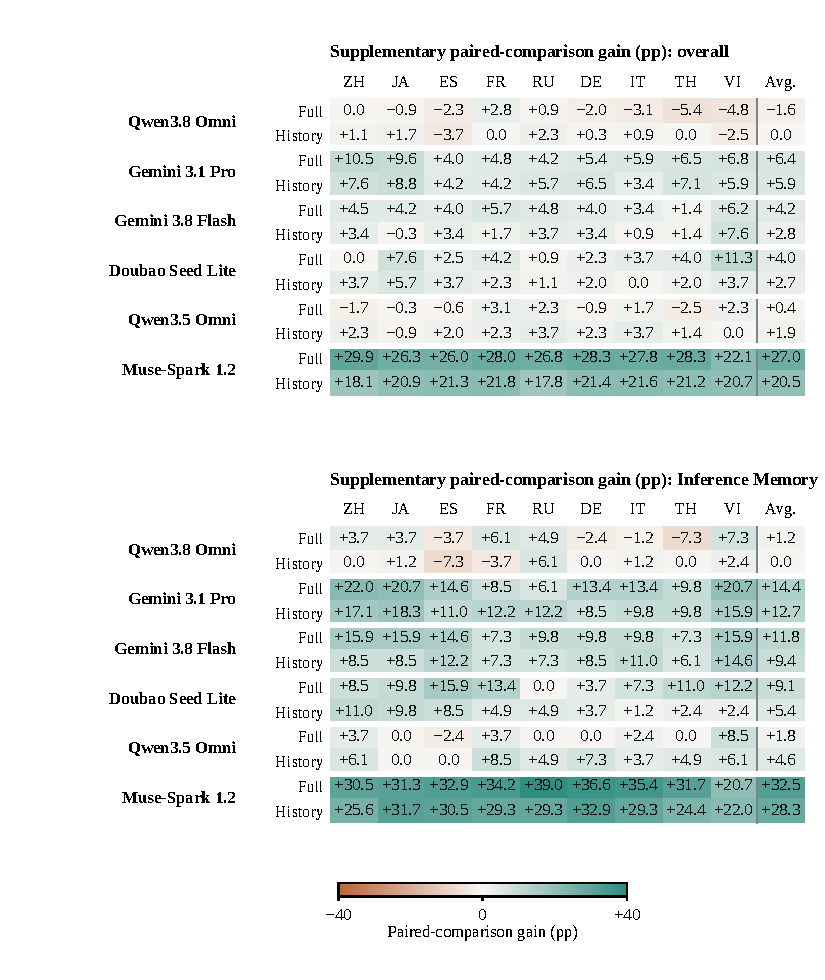
\includegraphics[width=\linewidth]{figures/transcription_gains_all_models.pdf}

\caption{Full-model comparison of Full Transcript and History Transcript paired instance-level gains over Direct Audio. Each model has Full and History rows; the two panels show overall and IM gains. Each procedure uses its own common samples and baseline. Avg. is the equal-weight mean of the nine non-English language gains (the paired export has no English arm). Signed values and an orange--teal scale distinguish losses and gains. These pairwise estimates are separate from the four-condition marginal contrasts in Table~\ref{tab:input_conditions}. These are descriptive point estimates.}

\label{fig:all_transcription_gains}

\end{figure}
